\section{Paper Visualization}
\label{appendix:paper_viz}

\subsection{Side-by-Side (SxS) Paper Visualizations}
\label{appendix:paper_viz_sxs}
In this section, we present full manuscript generation results for two samples (one from CVPR~\citep{bahari2025certified} and one from ICLR~\citep{drakulic2025goalgeneralistcombinatorialoptimization}) from \ourdataset{}. For each sample, we display the manuscripts generated from the original papers' raw materials under the sparse idea setting. We compare the final outputs produced by Single Agent, AI Scientist-v2, \ourmethod{} (PlotOff), and \ourmethod{} (PlotOn).


% ==========================================
% CVPR SAMPLE VISUALIZATIONS
% ==========================================

\begin{figure}[htbp]
  \centering
  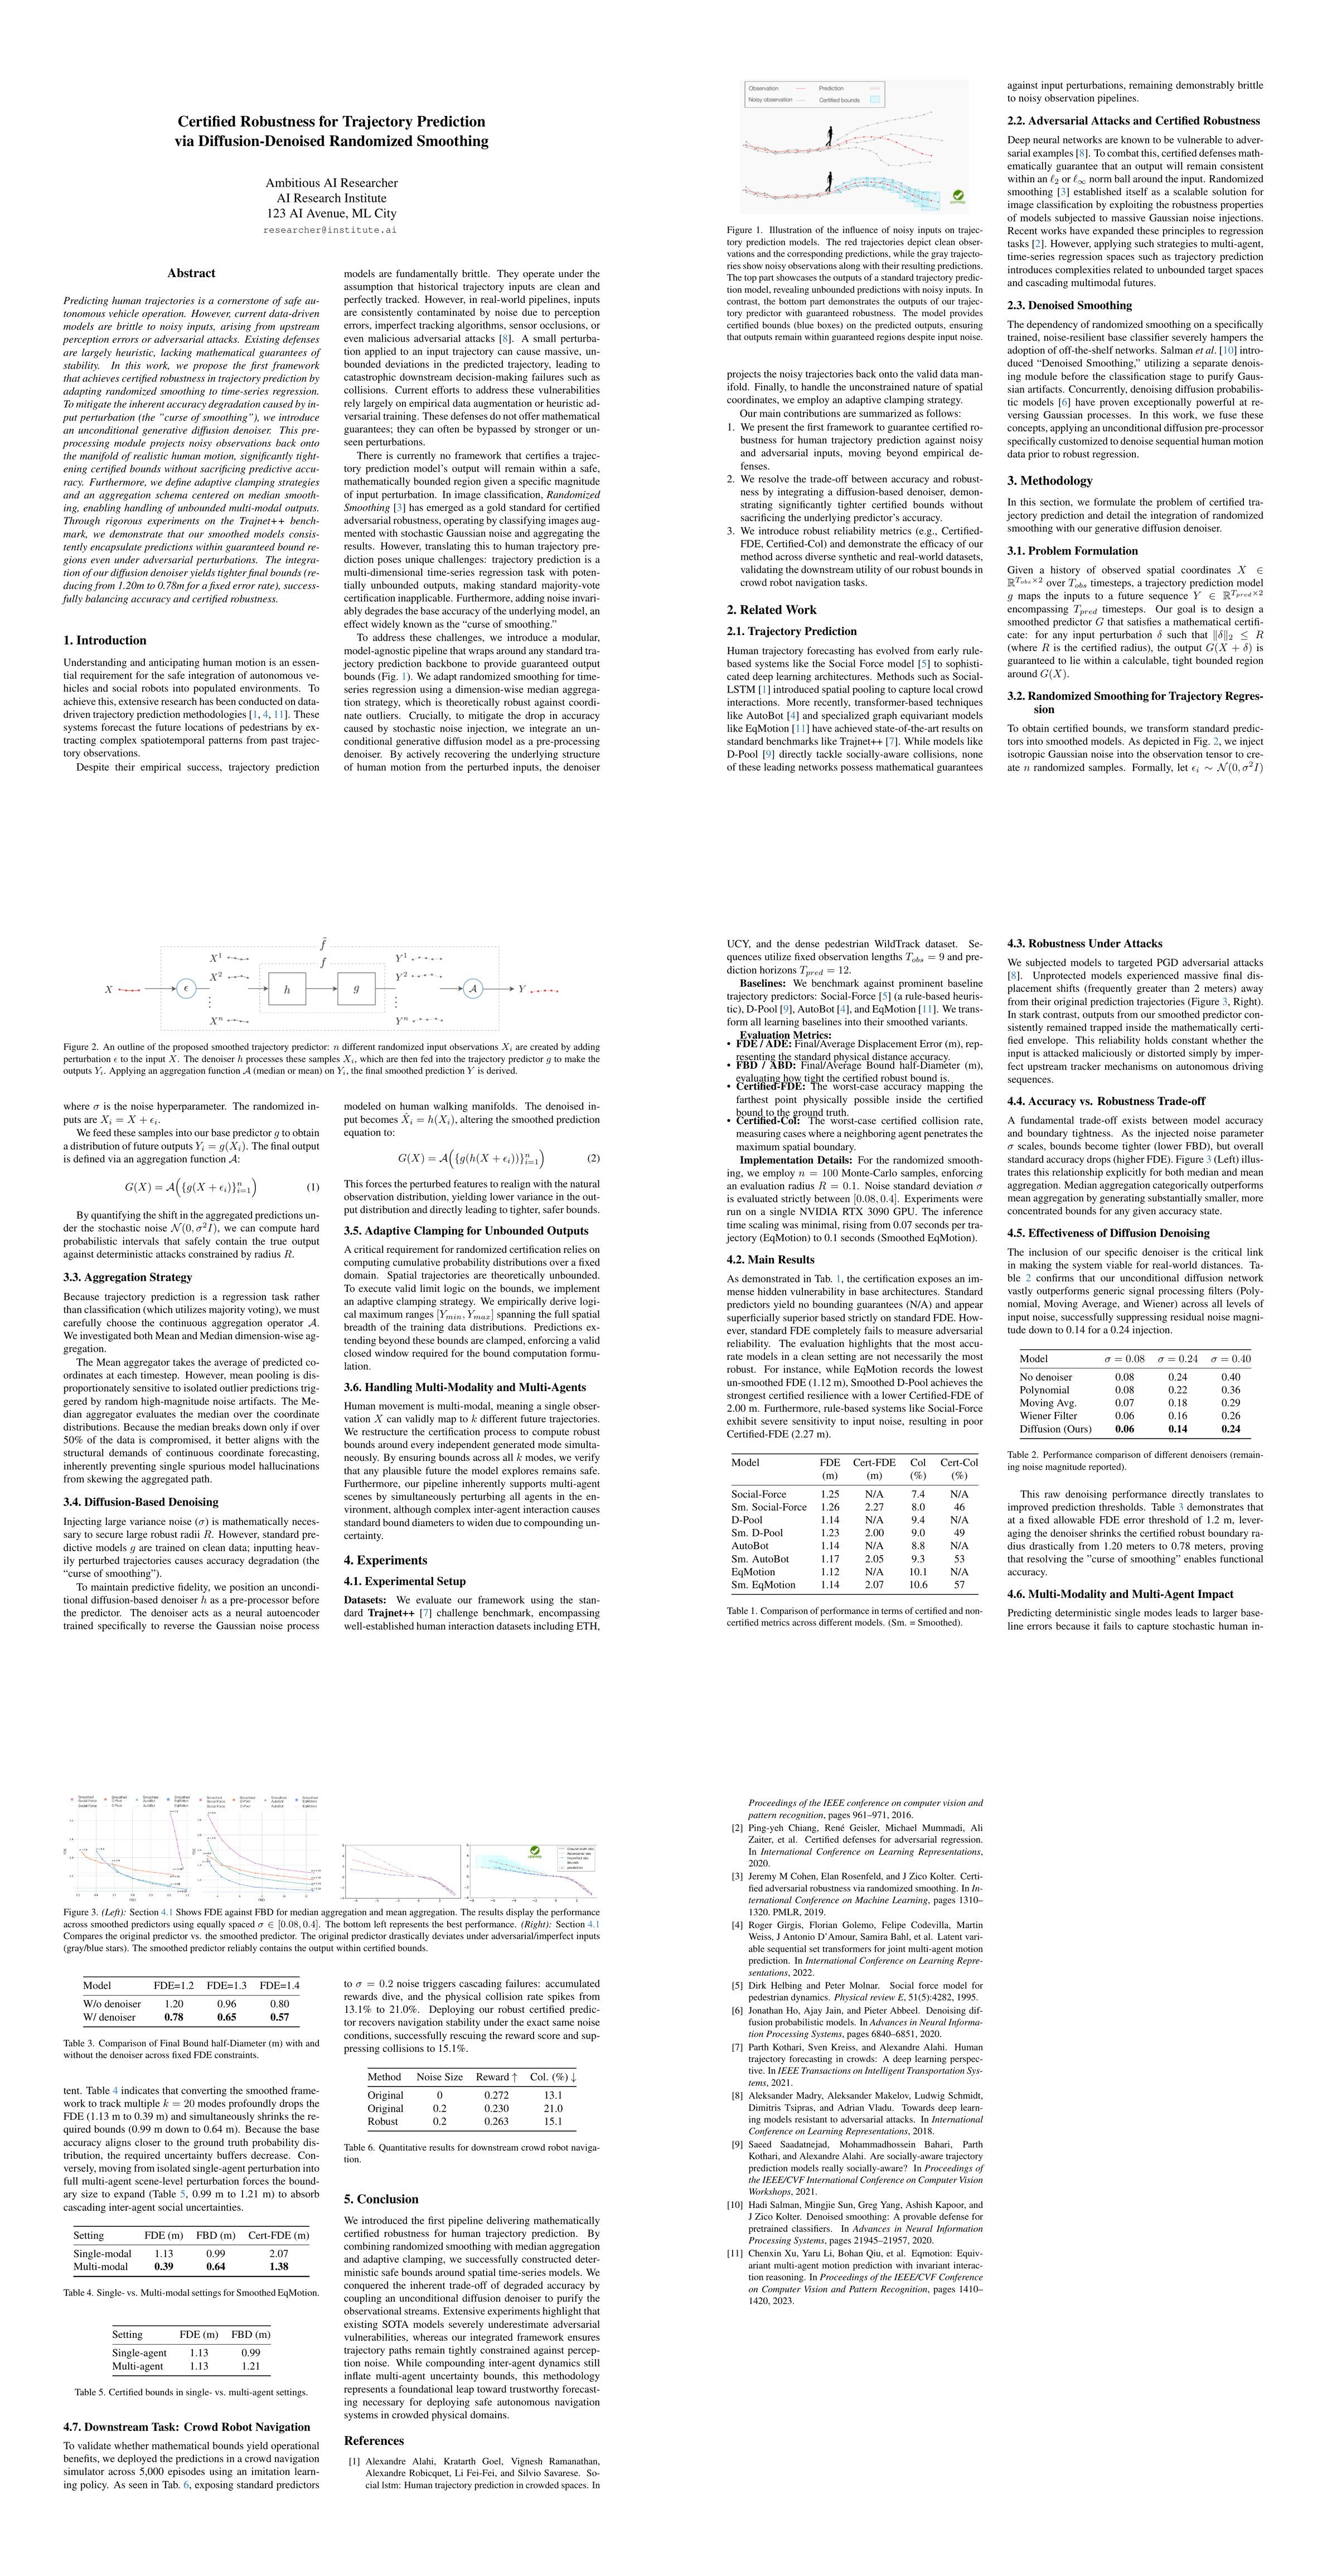
\includegraphics[width=\textwidth, height=0.72\textheight, keepaspectratio]{content/figures/paper_viz_sxs/cvpr2025_5f3288a486/single_agent.jpg}
  \caption{\textbf{CVPR Sample (Single Agent).} Manuscript generated by the Single Agent baseline from raw materials under the sparse idea setting.}
  \label{fig:sxs_cvpr_single_agent}
\end{figure}

\clearpage

\begin{figure}[p]
  \centering
  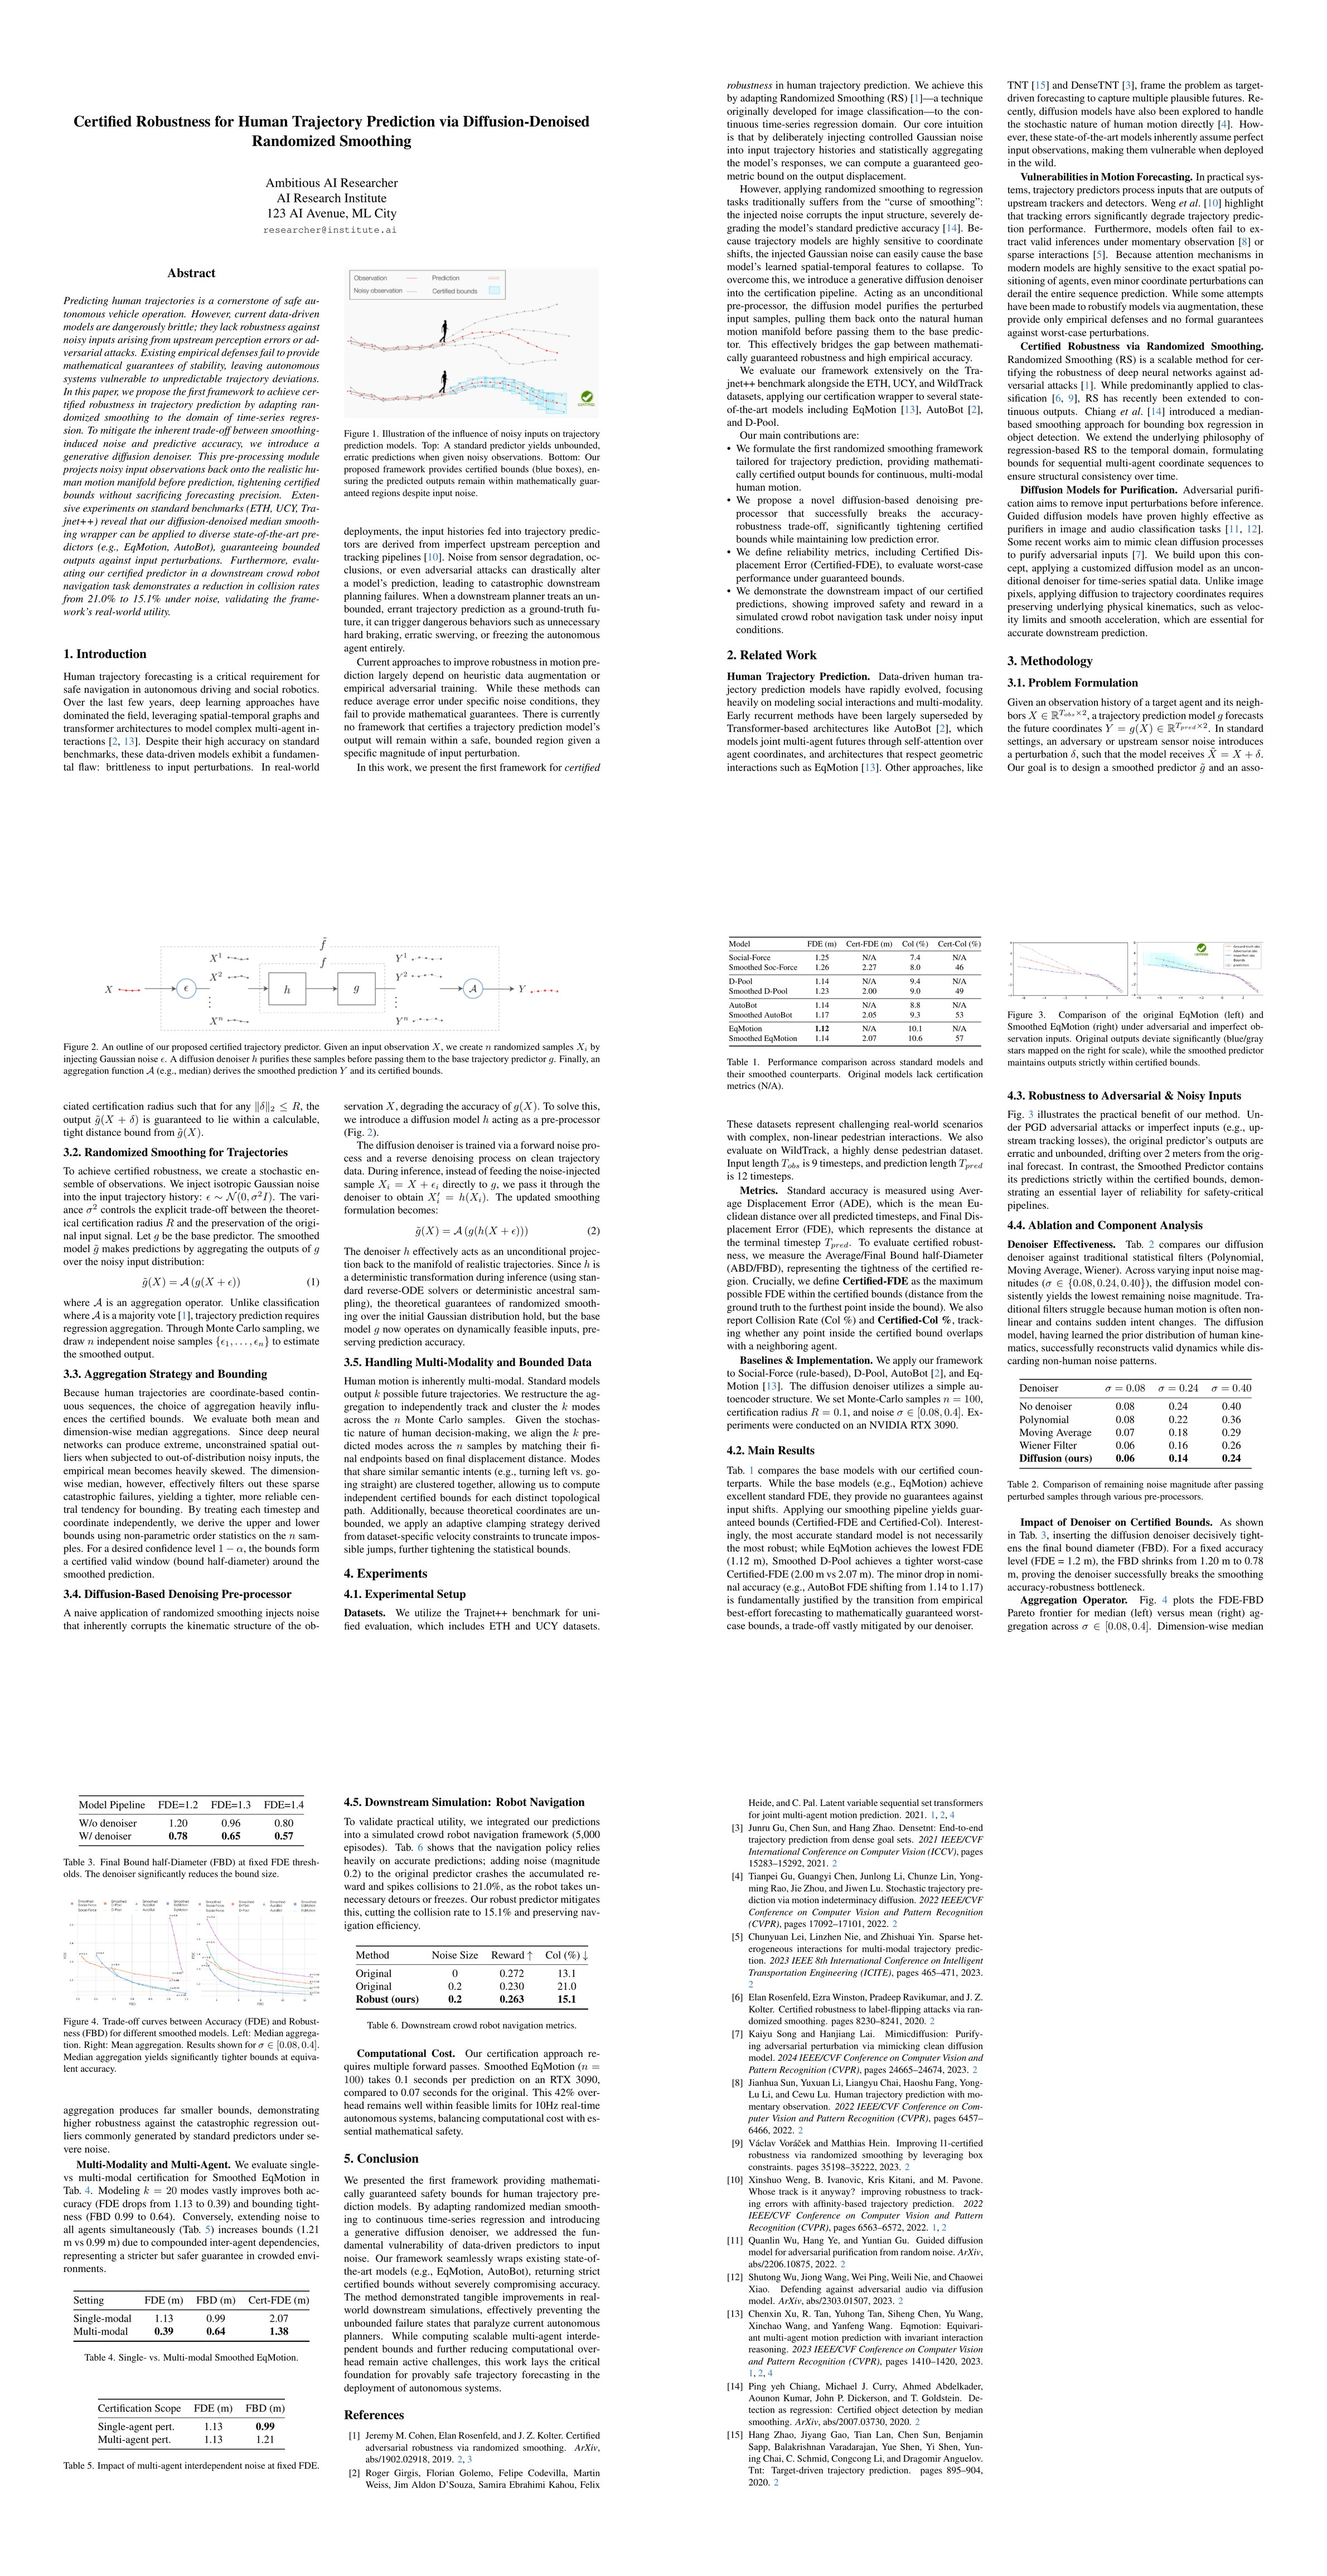
\includegraphics[width=\textwidth, height=0.85\textheight, keepaspectratio]{content/figures/paper_viz_sxs/cvpr2025_5f3288a486/ai_scientist.jpg}
  \caption{\textbf{CVPR Sample (AI Scientist-v2).} Manuscript generated by the AI Scientist-v2 baseline from raw materials under the sparse idea setting.}
  \label{fig:sxs_cvpr_ai_scientist}
\end{figure}

\clearpage

\begin{figure}[p]
  \centering
  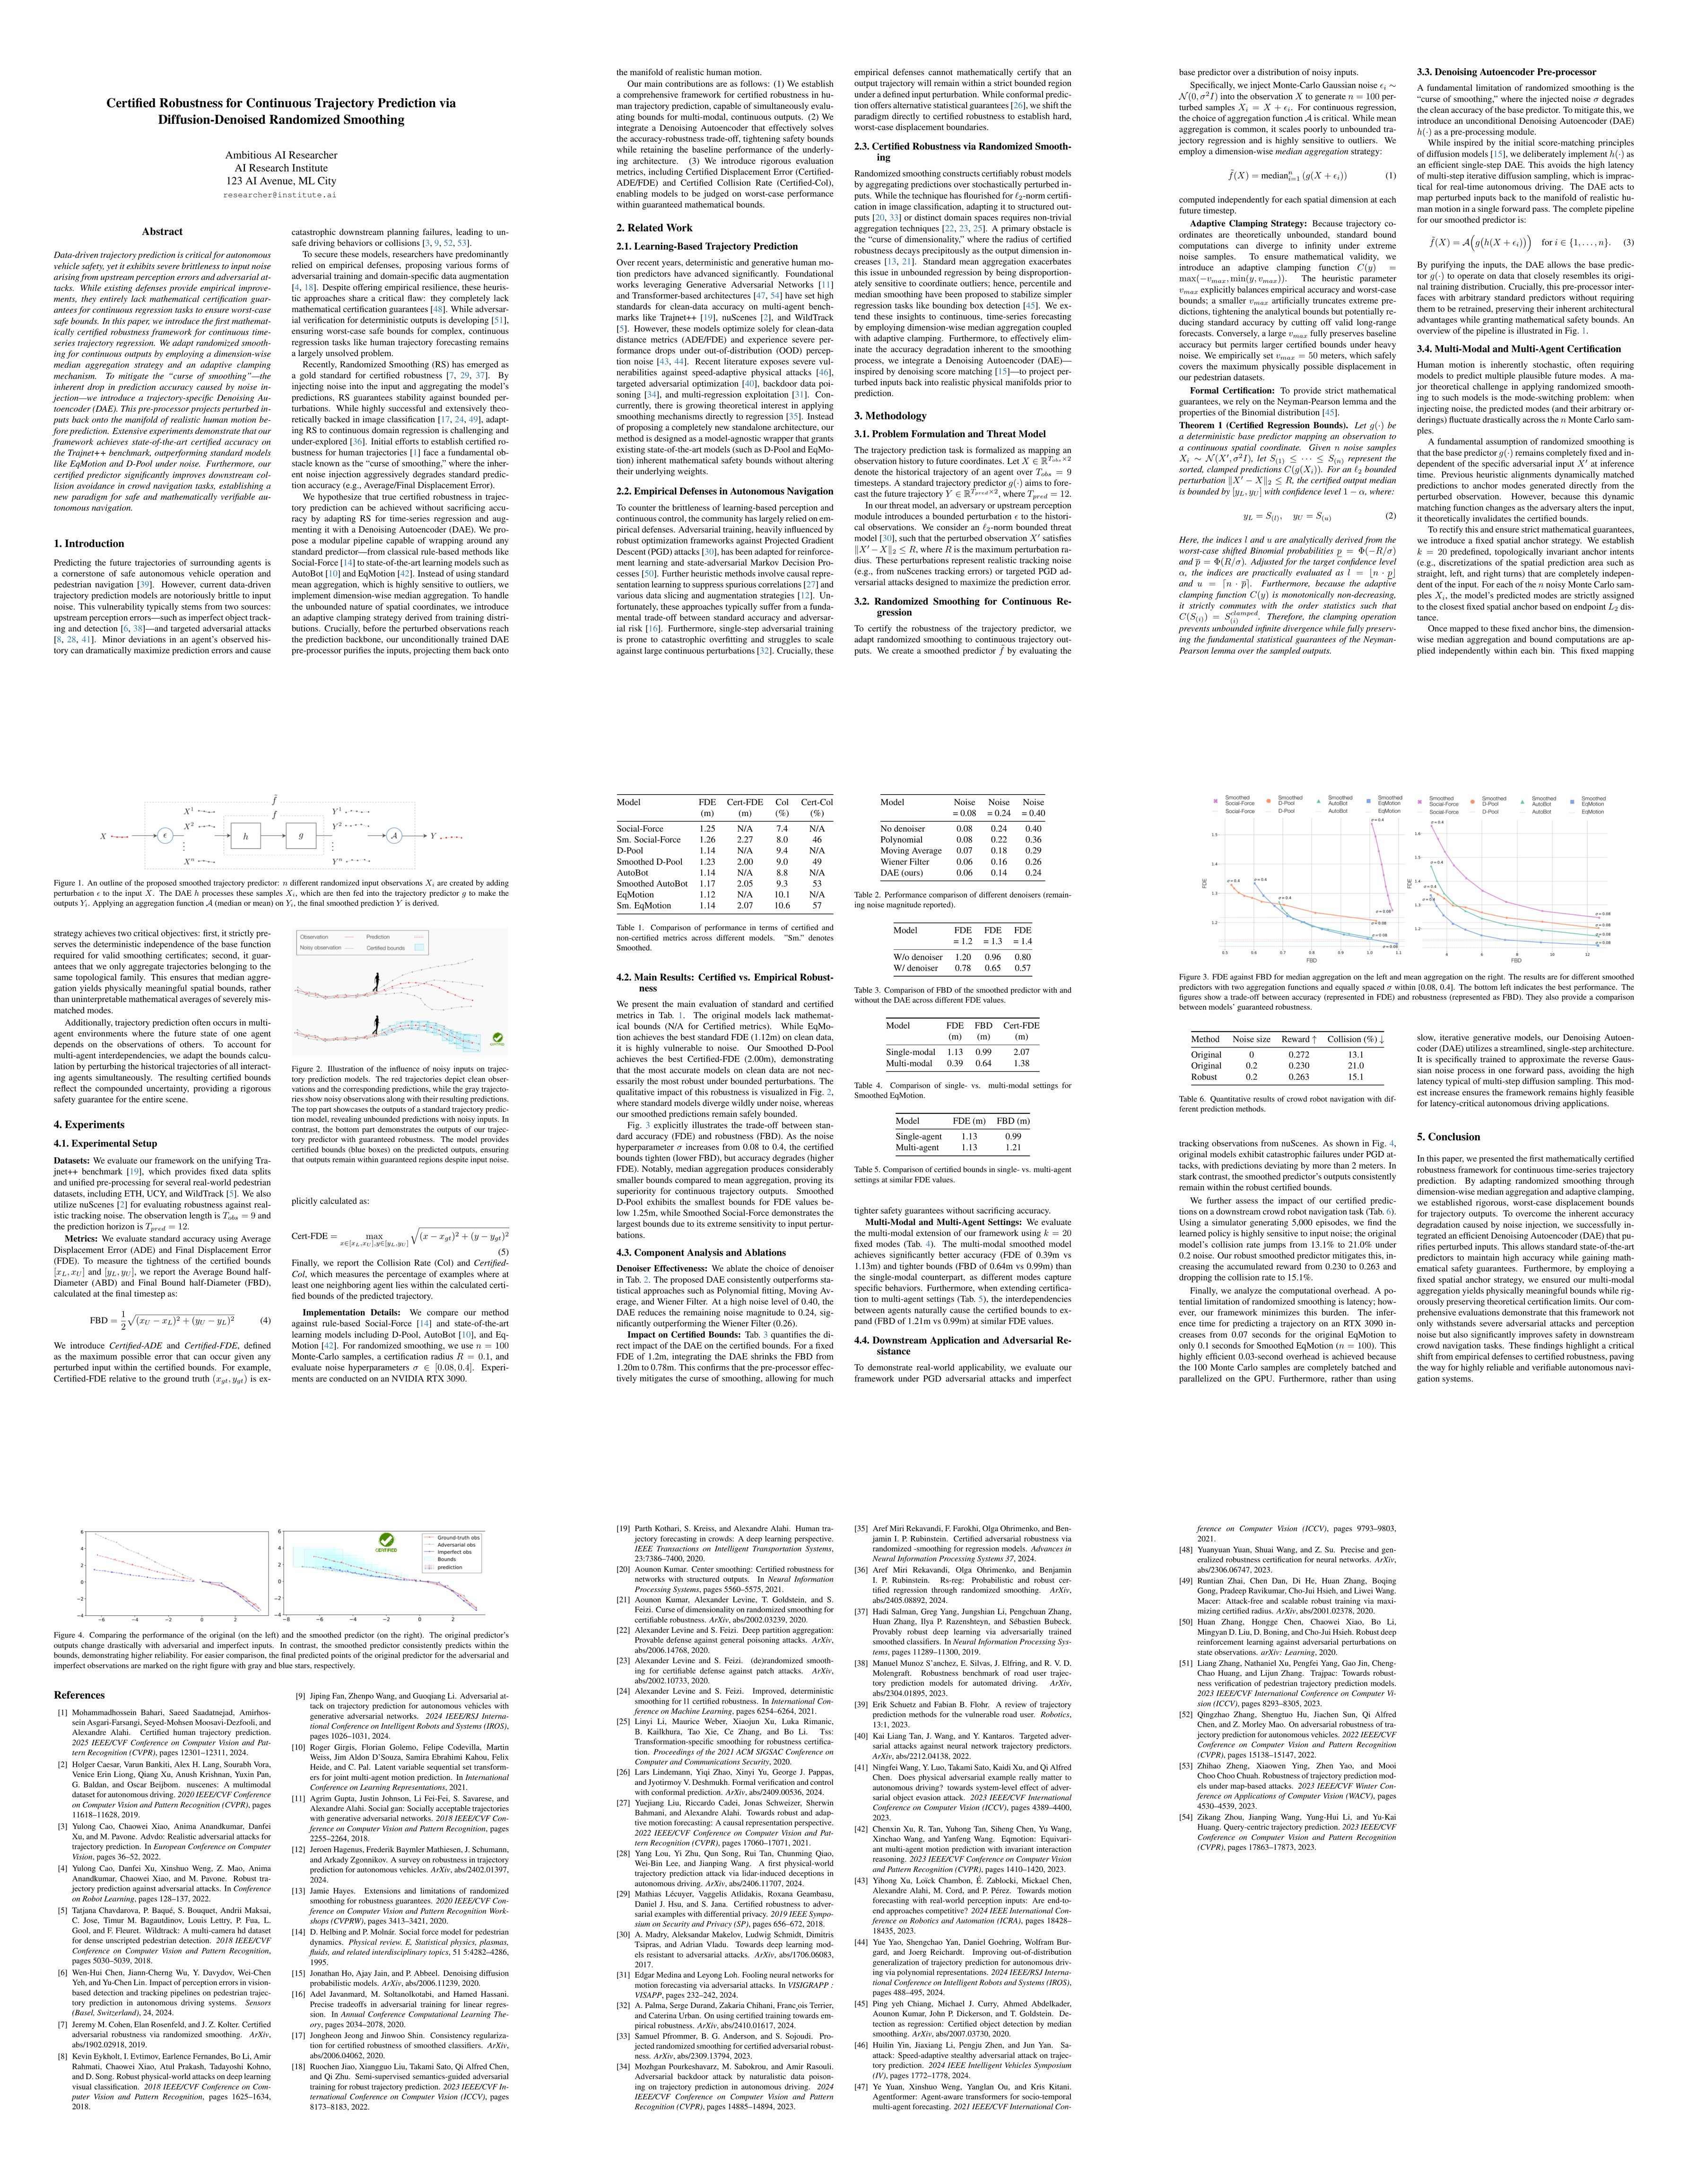
\includegraphics[width=\textwidth, height=0.85\textheight, keepaspectratio]{content/figures/paper_viz_sxs/cvpr2025_5f3288a486/ours_plotoff.jpg}
  \caption{\textbf{CVPR Sample (\ourmethod{} - PlotOff).} Manuscript generated by \ourmethod{} (PlotOff) from raw materials under the sparse idea setting.}
  \label{fig:sxs_cvpr_ours_plotoff}
\end{figure}

\clearpage

\begin{figure}[p]
  \centering
  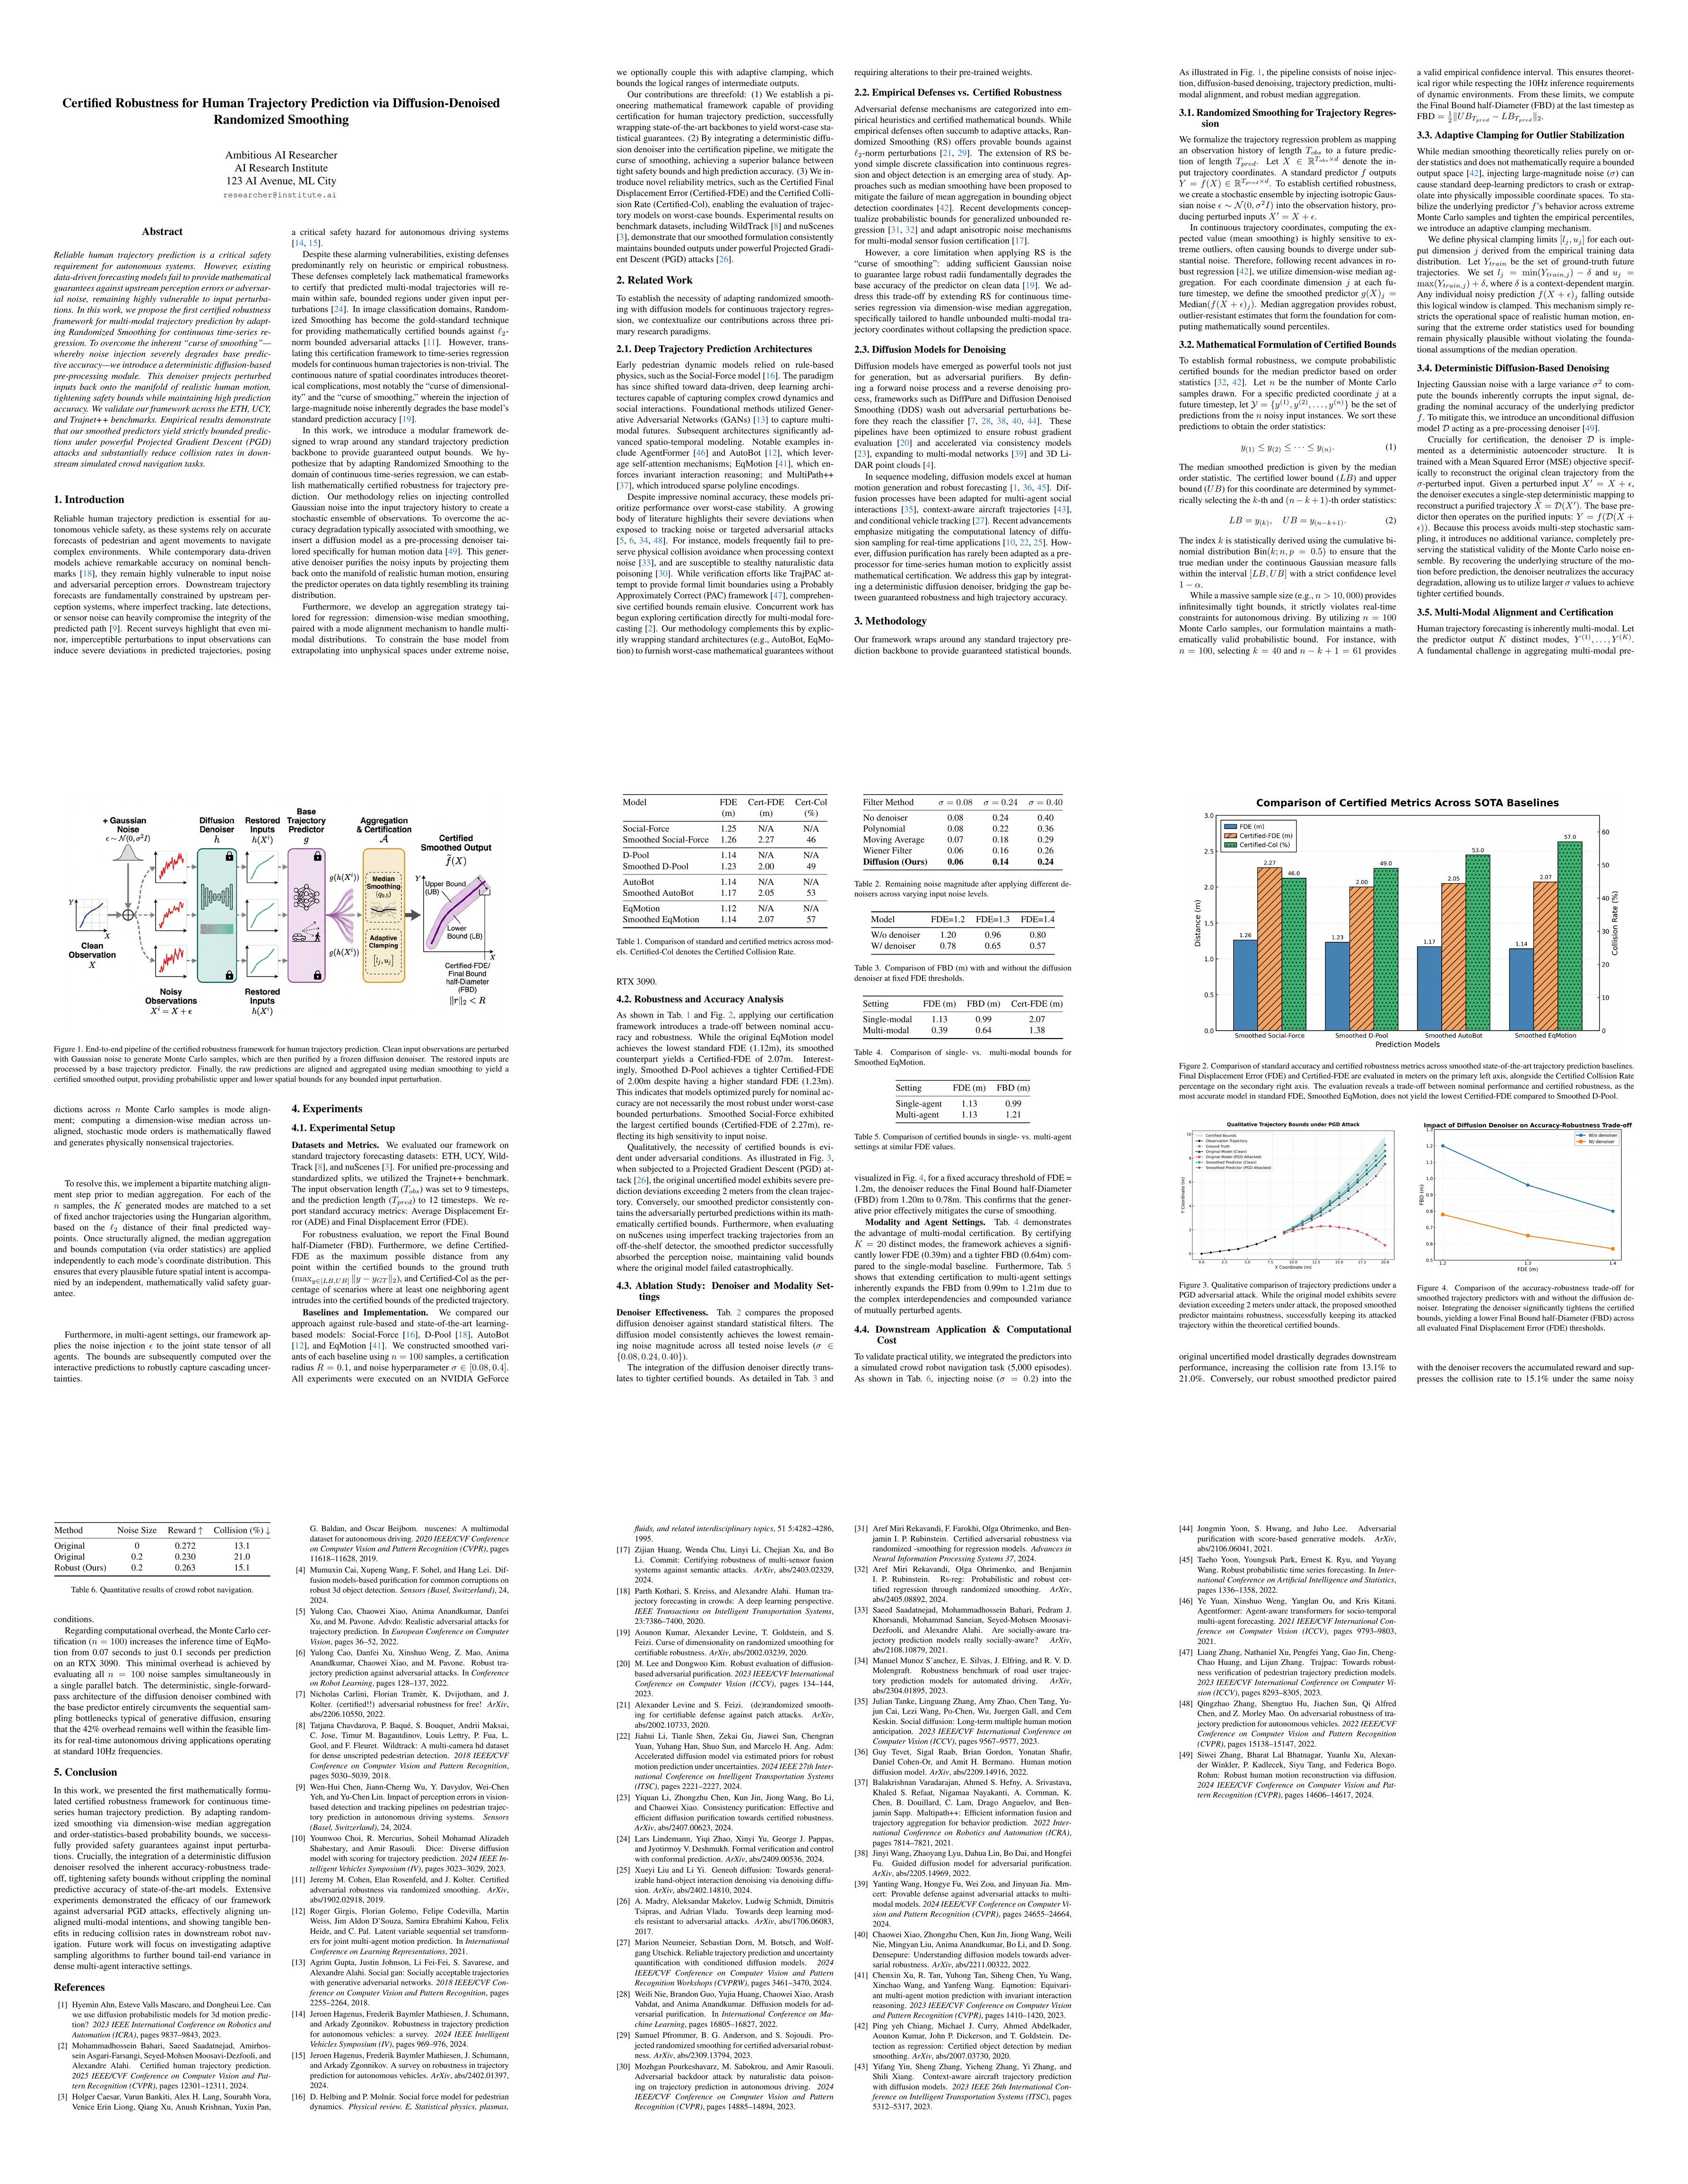
\includegraphics[width=\textwidth, height=0.85\textheight, keepaspectratio]{content/figures/paper_viz_sxs/cvpr2025_5f3288a486/ours_ploton.jpg}
  \caption{\textbf{CVPR Sample (\ourmethod{} - PlotOn).} Manuscript generated by \ourmethod{} (PlotOn) from raw materials under the sparse idea setting.}
  \label{fig:sxs_cvpr_ours_ploton}
\end{figure}

\clearpage

% ==========================================
% ICLR SAMPLE VISUALIZATIONS
% ==========================================

\begin{figure}[p]
  \centering
  
\includegraphics[width=\textwidth, height=0.85\textheight, keepaspectratio]{content/figures/paper_viz_sxs/iclr2025_b3bf83134b/single_agent.jpg}
  \caption{\textbf{ICLR Sample (Single Agent).} Manuscript generated by the Single Agent baseline from raw materials under the sparse idea setting.}
  \label{fig:sxs_iclr_single_agent}
\end{figure}

\clearpage

\begin{figure}[p]
  \centering
  
\includegraphics[width=\textwidth, height=0.85\textheight, keepaspectratio]{content/figures/paper_viz_sxs/iclr2025_b3bf83134b/ai_scientist.jpg}
  \caption{\textbf{ICLR Sample (AI Scientist-v2).} Manuscript generated by the AI Scientist-v2 baseline from raw materials under the sparse idea setting.}
  \label{fig:sxs_iclr_ai_scientist}
\end{figure}

\clearpage

\begin{figure}[p]
  \centering
  
\includegraphics[width=\textwidth, height=0.85\textheight, keepaspectratio]{content/figures/paper_viz_sxs/iclr2025_b3bf83134b/ours_plotoff.jpg}
  \caption{\textbf{ICLR Sample (\ourmethod{} - PlotOff).} Manuscript generated by \ourmethod{} (PlotOff) from raw materials under the sparse idea setting.}
  \label{fig:sxs_iclr_ours_plotoff}
\end{figure}

\clearpage

\begin{figure}[p]
  \centering
  
\includegraphics[width=\textwidth, height=0.85\textheight, keepaspectratio]{content/figures/paper_viz_sxs/iclr2025_b3bf83134b/ours_ploton.jpg}
  \caption{\textbf{ICLR Sample (\ourmethod{} - PlotOn).} Manuscript generated by \ourmethod{} (PlotOn) from raw materials under the sparse idea setting.}
  \label{fig:sxs_iclr_ours_ploton}
\end{figure}

\clearpage

\subsection{Sparse vs. Dense Idea Settings}
\label{appendix:paper_viz_sparse_dense}

To illustrate how input granularity influences technical depth, we contrast the methodology text synthesized by \ourmethod{} under the Sparse and Dense settings using a sample from the ICLR split~\citep{drakulic2025goalgeneralistcombinatorialoptimization}. While the Sparse setting produces a conceptual, high-level overview of the architecture, the Dense setting grounds the methodology in formal mathematical notation, explicitly defining the state space (e.g., BQ-MDPs) and the underlying operations.

\begin{methodologybox}[Generated Methodology (Sparse Idea)]
\noindent To overcome the specialization bottleneck in Neural Combinatorial Optimization (NCO), we design a unified architecture comprising a shared central backbone and lightweight, problem-specific adapters. Our approach decouples the semantic formulation of individual optimization tasks from the core reasoning process, enabling a single model to learn a transferable meta-heuristic. 

\vspace{1em}
\noindent\textbf{Modular Input/Output via Shared Codebooks}
\vspace{0.5em}

\noindent Combinatorial optimization problems present diverse state spaces, including varying node features (e.g., coordinates, demands, time windows) and edge attributes (e.g., distances, precedence constraints). To bridge the gap between these distinct definitions and our unified backbone, we employ task-specific linear adapters. For a given task, node features $x_i$ and edge features $e_{ij}$ are linearly projected into low-dimensional spaces: $h_i \in \mathbb{R}^8$ and $g_{ij} \in \mathbb{R}^4$, respectively. 

\vspace{0.5em}
\noindent To ensure that representations from different tasks are mapped into compatible subspaces within the backbone, we enforce a representational bottleneck using a shared codebook. The codebook acts as a continuous projection matrix $C \in \mathbb{R}^{8 \times 128}$ for nodes and $\bar{C} \in \mathbb{R}^{4 \times 128}$ for edges, mapping the low-dimensional task features into the high-dimensional embedding space of the backbone ($D=128$). The projected node embeddings $\hat{h}_i = h_i C$ and edge embeddings $\hat{g}_{ij} = g_{ij} \bar{C}$ force the model to learn a common vocabulary across all tasks, preventing catastrophic interference during multi-task training.

\vspace{1em}
\noindent\textbf{Mixed-Attention Mechanism}
\vspace{0.5em}

\noindent Standard Transformers excel at modeling node-to-node interactions but struggle to natively incorporate edge-level constraints, which are critical in routing and scheduling. Instead of relying on structural positional encodings, we introduce a \textit{Mixed-Attention} block that dynamically integrates edge information directly into the attention mechanism. 

\vspace{0.5em}
\noindent For each attention head, the query $q_i$, key $k_j$, and value $v_j$ are computed from the node embeddings $\hat{h}_i$. Simultaneously, the edge embeddings $\hat{g}_{ij}$ are transformed into edge-specific keys $k^{(e)}_{ij}$ and values $v^{(e)}_{ij}$. The affinity score between node $i$ and node $j$ is computed by additively combining the node-to-node interactions with the edge features:
\[
    A_{ij} = \text{softmax} \left( \frac{q_i^\top k_j + q_i^\top k^{(e)}_{ij}}{\sqrt{d_k}} \right)
\]
where $d_k$ is the dimensionality of the key vectors. The output of the attention head is then given by $\sum_j A_{ij} (v_j + v^{(e)}_{ij})$. This mechanism allows the model to dynamically weigh the importance of relationships based on explicit edge attributes (e.g., asymmetric distances or temporal constraints). The backbone consists of 9 such layers with 8 attention heads and a feed-forward dimension of 512, regularized via ReZero.

\vspace{1em}
\noindent\textbf{Multi-Type Transformer Architecture}
\vspace{0.5em}

\noindent Many scheduling problems, such as the Job Shop Scheduling Problem (JSSP), are defined on multipartite graphs involving heterogeneous entities (e.g., jobs vs. machines). Treating these distinct entities uniformly as generic nodes strips away crucial semantic information. To address this, we propose a \textit{Multi-Type} architecture. 

\vspace{0.5em}
\noindent When processing a graph with multiple node types, the Mixed-Attention blocks are duplicated to handle specific structural relationships (e.g., job-to-job, job-to-machine, machine-to-machine). Crucially, to maintain the generalist nature of the backbone and prevent parameter explosion, these duplicated blocks strictly share the same parameters. The network dynamically routes computations through the appropriate relation-specific blocks based on the node types present in the current task. This parameter-sharing constraint enables the backbone to process complex, multi-modal graph structures without requiring specialized modules for every new topological configuration.

\vspace{1em}
\noindent\textbf{Multi-Task Imitation Learning Strategy}
\vspace{0.5em}

\noindent We train GOAL in a multi-task setting using Imitation Learning. We generate expert trajectories across diverse problem classes using classical oracle solvers. The model is trained to autoregressively construct solutions, effectively framing optimization as a sequential generation task. 

\vspace{0.5em}
\noindent For tasks requiring a permutation of nodes (e.g., ATSP, CVRP), we apply a standard cross-entropy loss over the predicted probability distribution of the next node. For tasks involving multiple simultaneous decisions (e.g., Knapsack, MVC), we utilize a multi-class cross-entropy loss. The unified backbone is optimized end-to-end using the AdamW optimizer with an initial learning rate of $0.0005$, decayed by a factor of $0.97$ every 10 epochs.
\end{methodologybox}

\begin{methodologybox}[Generated Methodology (Dense Idea)]
\noindent We formulate the solution to multi-task combinatorial optimization as a constructive sequential decision-making process. The multi-task environment is defined as a disjoint union of Bisimulation Quotient Markov Decision Processes (BQ-MDPs), where states correspond to problem instances and actions correspond to construction steps (e.g., sequential node selections). To process highly variable environments within a single framework, GOAL decouples task-specific feature mapping from a shared reasoning backbone.

\vspace{1em}
\noindent\textbf{Task Representation and Input Adapters}
\vspace{0.5em}

\noindent For any given task $t$, we define an instance formally as a tuple $(x, \bar{x})$. Here, $x \in \mathbb{R}^{N \times F_t}$ represents the feature vectors of $N$ nodes with task-specific dimension $F_t$, and $\bar{x} \in \mathbb{R}^{N \times N \times \bar{F}_t}$ represents the feature vectors of edges with dimension $\bar{F}_t$. 

\vspace{0.5em}
\noindent Because different problems exhibit varying initial feature dimensions, we map these variables to a shared backbone embedding dimension $D$ using Task-Specific Adapters combined with a Shared Linear Projection. To prevent isolated subspace specialization, we enforce low-rank projections:

\vspace{0.5em}
\noindent 1. \textbf{Input Adapter:} A task-specific linear layer maps the raw inputs down to a low-dimensional space $\ell \ll D$.

\vspace{0.5em}
\noindent 2. \textbf{Shared Linear Projection:} A universally learnable matrix of size $\ell \times D$ projects this compressed representation into the shared backbone space. (Note: this component is labeled as a `codebook' in figures for visual brevity, though it acts purely as a continuous linear projection and not a discrete quantization dictionary).

\vspace{1em}
\noindent\textbf{Multi-Head Mixed-Attention Mechanism}
\vspace{0.5em}

\noindent The core reasoning engine of GOAL is a Transformer stack utilizing a Multi-Head Mixed-Attention mechanism. Unlike standard transformers that rely solely on node features, our mechanism natively ingests edge features $\bar{x}$ directly into the attention score computation. 

\vspace{0.5em}
\noindent For a given attention head $h$, let $M$ be the number of query nodes and $N$ be the number of key/value nodes. The standard projections for node queries ($Q$), keys ($K$), and values ($V$) are defined as:
\[
Q_n^{(h)} = Q_n \mathbf{W}_Q^{(h)}, \quad K_m^{(h)} = K_m \mathbf{W}_K^{(h)}, \quad V_m^{(h)} = V_m \mathbf{W}_V^{(h)}
\]
Simultaneously, we define projections for the edge features $E_{mn}$ (derived from $\bar{x}$) into the query and key spaces:
\[
Q_{mn}^{\prime (h)} = E_{mn} \mathbf{W}_Q^{\prime (h)}, \quad K_{mn}^{\prime (h)} = E_{mn} \mathbf{W}_K^{\prime (h)}
\]
The attention scores $S_{mn}^{(h)}$ are then computed by adding the edge-derived vectors to the node-derived vectors \textit{before} the scalar product:
\[
S_{mn}^{(h)} = \langle K_m^{(h)} + K_{mn}^{\prime (h)} \mid Q_n^{(h)} + Q_{mn}^{\prime (h)} \rangle
\]
This formulation structurally integrates relational data without incurring computational overhead when such features are absent, as the edge terms simply evaluate to zero. 

\vspace{0.5em}
\noindent While our mechanism shares mathematical foundations with relative positional encodings and other edge-augmented models, it fundamentally differs in application. Instead of learning 1D scalar biases based on graph distance, our Mixed-Attention dynamically projects dense, multi-dimensional asymmetric edge features (such as explicit transition costs or capacity constraints) directly into the high-dimensional query and key vector spaces before the scalar product. 

\vspace{1em}
\noindent\textbf{Multi-Type Transformer Architecture}
\vspace{0.5em}

\noindent To handle combinatorial problems defined on heterogeneous graphs (e.g., bipartite connections mapping ``Jobs'' to ``Machines'' in scheduling tasks), we extend the backbone into a Multi-Type Architecture. Rather than padding disparate types into a single homogeneous tensor, we dynamically compose layer operations based on the inherent task structure.

\vspace{0.5em}
\noindent We instantiate separate self-attention blocks for each distinct node type, and cross-attention blocks for valid type pairings. Crucially, to maintain the generalist nature of the model, all attention blocks within a specific layer share the \textit{exact same parameters} ($\mathbf{W}_Q, \mathbf{W}_K, \mathbf{W}_V$, etc.), regardless of whether they are performing self-attention or cross-attention. This forces disparate graph typologies to map into a unified algorithmic reasoning space.

\vspace{0.5em}
\noindent One might consider an alternative approach: concatenating all nodes into a single sequence and utilizing a block-sparse attention mask. However, standard transformers with sparse masks often still allocate memory-intensive full-sequence tensors ($N \times N$) before applying the mask. Our Multi-Type architecture avoids this by explicitly instantiating structured attention blocks \textit{only} for valid topological pairings, bypassing the quadratic computational waste associated with invalid interactions. 

\vspace{1em}
\noindent\textbf{Training Protocol and Decoding}
\vspace{0.5em}

\noindent GOAL is trained in a multi-task setting via Imitation Learning. To train the model, we require step-by-step constructive trajectories derived from optimal or highly optimized heuristic oracles. 

\vspace{0.5em}
\noindent \textbf{Trajectory Canonicalization:} For sequential routing tasks with bidirectional symmetries (e.g., the TSP, where a forward and backward tour represent the same cycle), we canonicalize the expert trajectories to prevent conflicting teaching signals. We enforce a fixed traversal direction by always starting at the depot and breaking initial directional ties by visiting the lowest-indexed node first.

\vspace{0.5em}
\noindent For unordered tasks such as the Knapsack Problem (KP) and Minimum Vertex Cover (MVC), expert solvers output static sets of selected items. To convert these into sequential trajectories without masking optimal items, we take the exact optimal subset $S^*$ provided by the oracle, and strictly order \textit{only} the elements within $S^*$ by a defined heuristic (e.g., value-to-weight ratio for KP, residual degree for MVC). This translates the unordered solution into a deterministic, valid trajectory that the policy can effectively imitate.

\vspace{0.5em}
\noindent We minimize the cross-entropy loss between the model's predicted action probabilities and these optimal trajectories. A task-specific linear projection maps the final backbone output to a score matrix representing the log-logits for valid node selection. A softmax operation is then applied over the dynamically updated valid action mask to yield the final policy distribution.

\vspace{0.5em}
\noindent \textbf{Autoregressive Decoding and Efficiency:} To maintain fast inference times scaling up to 1000-node instances, GOAL does \textit{not} re-evaluate the entire Transformer backbone at every autoregressive step. Instead, the heavy 9-layer backbone processes the static graph features (e.g., node coordinates, distance matrices) exactly once, caching the high-dimensional node and edge embeddings. At each constructive step, a lightweight Output Adapter takes the cached embeddings along with the rapidly changing dynamic state features (e.g., current location, remaining vehicle capacity) to compute the next valid action. This cached decoding strategy prevents quadratic recalculations at each step.
\end{methodologybox}